% Gerado por Texto-TCC/gerar-latex.pl a partir de Artigo-TCC1-NeuroSight.md em 10/11/2026.
% Para mudar o texto, edite os arquivos das seções em Texto-TCC, monte o artigo com
% montar-artigo.pl e gere de novo este arquivo; mudanças feitas direto aqui se perdem na próxima geração.
% O preâmbulo e a capa seguem o textoprincipal.tex do modelo do curso. Diferenças: a classe é
% IEEEtran (com t minúsculo, que também funciona no Overleaf), o pacote tabularx e o ambiente
% figuralarga, porque o figura* do tads.tex usa figure, que ocupa uma coluna só.
\documentclass[conference,a4paper,10pt]{IEEEtran}

\usepackage{amsmath,amssymb,amsfonts}
\usepackage{algorithmic}
\usepackage{graphicx}
\usepackage{textcomp}
\usepackage{xcolor}
\usepackage{multirow}
\usepackage{setspace}
\usepackage{pdfpages}
\usepackage{float}
\usepackage{caption,newfloat}
\usepackage[T1]{fontenc}
\usepackage[brazilian]{babel}
\usepackage[utf8]{inputenc}
\usepackage{ifthen}
\usepackage[pages=some]{background}
\usepackage{tabularx}
\RequirePackage[obeyspaces,hyphens]{url}
\RequirePackage[plainpages,pdfpagelabels]{hyperref}	% PDF com links, metadados
\RequirePackage{bookmark}				% cria um índice no PDF
\RequirePackage{microtype}	% melhorar a qualidade da tipografia no PDF

% coluna de tabela que quebra linha, alinhada à esquerda
\newcolumntype{Y}{>{\raggedright\arraybackslash}X}

%% Se alguma hifenização não funcionar, adicionar aqui
\hyphenation{di-gi-ta-li-za-das}


%%%%%%%%%%%%%%%%%%%%%%%%%%%%%%%%%%%%%%%%%%%%%%%%%%%%%%%%%%%%%%%%%%%%%%%%
%     INÍCIO DO DOCUMENTO
%%%%%%%%%%%%%%%%%%%%%%%%%%%%%%%%%%%%%%%%%%%%%%%%%%%%%%%%%%%%%%%%%%%%%%%%
\begin{document}

%%%% NÃO MEXER NESTES ARQUIVOS
%%%% Definições/Estilos customizadas para o TADS, Mais capa
% \captionsetup{
%    tablename=TABELA,
%    listformat=empty,
%    justification=centering,
%    %labelsep=newline,
%    position=above,
%    skip=0.2\baselineskip,
%    width=\linewidth,
%    labelfont={small},
%    font={small} 
% }

\newcommand{\legenda}[1]{\caption{#1}}

\pagenumbering{arabic}

\def\BibTeX{{\rm B\kern-.05em{\sc i\kern-.025em b}\kern-.08em
    T\kern-.1667em\lower.7ex\hbox{E}\kern-.125emX}}

\newcommand{\tabelaname}{TABELA}
\newcommand{\figuraname}{FIGURA}
\newcommand{\quadroname}{QUADRO}
\newcounter{quadrocounter}
\setcounter{quadrocounter}{0}
% posicao, legenda, fonte
\newenvironment{quadro}[4][!t]
{
  \refstepcounter{quadrocounter}
  \label{#4}
  \def\fonteval{#3}
  \begin{table}[#1]
    \begin{center}
      % legenda
      \par\medskip\noindent
      QUADRO~\thequadrocounter~-~#2
      \par\medskip\noindent
}
{
      \par\noindent
      \fonte{\fonteval}
    \end{center}
  \end{table}
}
\newenvironment{quadro*}[4][!t]
{
  \refstepcounter{quadrocounter}
  \label{#4}
  \def\fonteval{#3}
  \begin{table*}[#1]
    \begin{center}
      % legenda
      \par\medskip\noindent
      QUADRO~\thequadrocounter~-~#2
      \par\medskip\noindent
}
{
      \par\noindent
      \fonte{\fonteval}
    \end{center}
  \end{table*}
}

\newcounter{tabelacounter}
\setcounter{tabelacounter}{0}
\newenvironment{tabela}[4][!t]
{
  \refstepcounter{tabelacounter}
  \label{#4}
  \def\fonteval{#3}
  \begin{table}[#1]
    \begin{center}
      % legenda
      \par\medskip\noindent
      TABELA~\thetabelacounter~-~#2
      \par\medskip\noindent
}
{
      \par\noindent
      \fonte{\fonteval}
    \end{center}
  \end{table}
}
\newenvironment{tabela*}[3][!t]
{
  \refstepcounter{tabelacounter}
  \def\fonteval{#3}
  \begin{table*}[#1]
    \begin{center}
      % legenda
      \par\medskip\noindent
      TABELA~\thetabelacounter~-~#2
      \par\medskip\noindent
}
{
      \par\noindent
      \fonte{\fonteval}
    \end{center}
  \end{table*}
}
\newcounter{figuracounter}
\setcounter{figuracounter}{0}
\newenvironment{figura}[4][!t]
{
  \def\fonteval{#3}
  \refstepcounter{figuracounter}
  \label{#4}
  \begin{figure}[#1]
    \begin{center}
      % legenda
      \par\medskip\noindent
      FIGURA~\thefiguracounter~-~#2
      \par\medskip\noindent
}
{
    \par\noindent
    \fonte{\fonteval}
    \end{center}
  \end{figure}
}
\newenvironment{figura*}[4][!t]
{
  \refstepcounter{figuracounter}
  \label{#4}
  \def\fonteval{#3}
  \begin{figure}[#1]
    \begin{center}
    % legenda
    \par\medskip\noindent
    FIGURA~\thefiguracounter~-~#2
    \par\medskip\noindent
}
{
    \par\noindent
    \fonte{\fonteval}
  \end{center}
  \end{figure}
}

\newcommand*{\captionsource}[2]{%
  \caption[{#1}]{%
  \centering
    #1%
    \hspace{\linewidth}%
    FONTE: #2%
  }%
}

\newcommand*{\fonte}[1]{%
  \centering
  \small
  \vspace{1em}
  \hspace{\linewidth}%
  FONTE: #1%
}

\def\abstractname{Abstract: }


%%%%%%%%%%%% CONFIGURAÇÃO DA CAPA E FOLHA DE ROSTO %%%%%%%%%%%%%%

\def\descr{Trabalho de conclusão de curso apresentado ao
curso de graduação em Análise e
Desenvolvimento de Sistemas, Setor de Educação
Profissional e Tecnológica, Universidade Federal
do Paraná, como requisito parcial à obtenção do
título de tecnólogo}



%%%% fundo na capa

\backgroundsetup{
scale=1,
color=black,
opacity=0.4,
angle=0,
contents={%
  
\includegraphics[width=\paperwidth,height=\paperheight]{bg_capa.jpg}
  }%
}
%%%%


%%%%%%% Definição da capa e folha de rosto


%\fancypagestyle{frontmatter}{
%  \fancyhf{}
%}

%\fancypagestyle{plain}{
%  \fancyhf{}
%  \if@mainmatter
%    \if@twoside
%      \fancyhead[LE,RO]{\thepage}
%    \else
%      \fancyhead[R]{\thepage}
%    \fi
%  \fi
%}



\hypersetup{
  % pdftitle, author, etc definidos mais abaixo
%  bookmarks   = true,
%  pageanchor  = false,
  hypertexnames = false,
%  bookmarkstype = page,
  pdfview     = Fit,
  pdfborder   = {0 0 0},
  colorlinks  = false,
  linkcolor   = blue,
  anchorcolor = blue,
  citecolor   = blue,
  filecolor   = blue,
%  pagecolor   = blue,
  urlcolor    = blue
}




%\def\@advisor{}			% orientador
%\def\@coadvisor{}		% co-orientador
%\def\@local{}			% local
%\def\@descr{}			% descrição do documento
%\def\@pcs{}			% palavras-chave
%\def\@kws{}			% keywords


%\newcommand{\autorcapa}[1]{\def\@author{#1}}
%\renewcommand{\title}[1]{\def\@title{#1}}

% descrição do documento na folha de rosto
%\newcommand{\descr}[1]{\def\@descr{#1}}

% orientadores
%\newcommand{\advisor}[1]{\def\@advisor{#1}}
%\newcommand{\coadvisor}[1]{\def\@coadvisor{#1}}


% local (cidade)
%\newcommand{\local}[1]{\def\@local{#1}}

\newcommand{\capa}[1]
{
  % páginas iniciais não são numeradas
  %\pagestyle{empty}
  %\thispagestyle{empty}

  % ajustar tags do PDF final
  \hypersetup{
    pdftitle    = {\titulo},
    pdfproducer = {UFPR - Universidade Federal do Paraná}
  }

  % primeira capa (só na versão aprovada)
  %\iffinalmode
%    \phantomsection
%    \thispagestyle{empty}

    \BgThispage
    
    \begin{center}
      \begin{doublespace}
        \textsc{\Large{UNIVERSIDADE FEDERAL DO PARANÁ}}
        \par
        \vspace{2cm}
        #1
        \vfill
        \DeclareRobustCommand\\{\linebreak}
        \textsc{\Large\titulo}
        \vfill
        \textsc{\Large\local\\\ano}
      \end{doublespace}
    \end{center}
    \cleardoublepage
    
    
  %\fi

  % folha de rosto
  \clearpage
%  \phantomsection
%  \addcontentsline{toc}{chapter}{Rosto}
%  \thispagestyle{empty}

  % autor
  \begin{center}
      \begin{doublespace}
        #1
      \end{doublespace}
  \end{center}

  \vfill\vfill

  % título
  \begin{doublespace}
    \begin{center}
      \DeclareRobustCommand\\{\linebreak }
      \textsc{\Large\titulo}
    \end{center}
  \end{doublespace}

  \vspace{1cm}

  % selo descritivo
  \hfill
  \begin{minipage}{9cm}

    % descrição
    \ifx\descr\@empty
    \else
      \descr.
    \fi

    % orientador
    \ifx\orientador\@empty
    \else
      \vspace{1em}
      Orientador: \orientadornome.
    \fi

    % coorientador
    \ifx\coorientador\undefined
    \else
      \vspace{1em}
      Co-orientador: \coorientador.
    \fi

  \end{minipage}

  \vfill

  % local e data
  \begin{center}
    \begin{doublespace}
      \textsc{\Large\local\\\ano}
    \end{doublespace}
  \end{center}

  % that's all, folks!
  \cleardoublepage
}


\newcommand{\termoaprovacao}
{
    \begin{center}
      \begin{doublespace}
        \vfill
        \Large{Substituir esta página pelo Termo de Aprovação que será fornecido após a defesa.}
        \vfill
      \end{doublespace}
    \end{center}
    \cleardoublepage
    
}

% \newcommand{\linebreakand}{%
%   \end{@IEEEauthorhalign}
%   \hfill\mbox{}\par
%   \mbox{}\hfill\begin{@IEEEauthorhalign}
% }

\newcommand*{\refmark}[1]{\raisebox{0pt}[0pt][0pt]{\textsuperscript{\footnotesize #1}}}
\newcommand{\autores}[1]{
  \author{
      \IEEEauthorblockN{
        #1
      }
      %\IEEEauthorblockN{#1\refmark{1}, #2\refmark{1}, #3\refmark{1}, #4\refmark{1}, #5\refmark{1}}
      \IEEEauthorblockA{\refmark{1}\textit{\setor} \\ \textit{\ufpr} }
  }
}

%%%%%%%

\hypersetup{pdfauthor={João Vitor Zanini Pedro, Lucas Sarnacki Guiraud}}

% Figura na largura das duas colunas, com legenda e fonte como as do figura do tads.tex
\newenvironment{figuralarga}[4][!t]
{
  \refstepcounter{figuracounter}
  \label{#4}
  \def\fonteval{#3}
  \begin{figure*}[#1]
    \begin{center}
      \par\medskip\noindent
      FIGURA~\thefiguracounter~-~#2
      \par\medskip\noindent
}
{
      \par\noindent
      \fonte{\fonteval}
    \end{center}
  \end{figure*}
}

%%%%%%%%%%%%%%%%%%%%%%%%%%%%%%%%%%%%%%%%%%%%%%%%%%%%%%%%%%%%%%%%%%%%%%%%
%%%% Definições usadas para geração da capa, folha de rosto e títulos
\def\autorescapa{
    \textsc{\Large JOÃO VITOR ZANINI PEDRO}\\
    \textsc{\Large LUCAS SARNACKI GUIRAUD}\\
}
\def\autorestitulo{
  João Vitor Zanini Pedro\refmark{1}, Lucas Sarnacki Guiraud\refmark{1}
}
\def\titulo{NeuroSight: sistema de rastreamento ocular e emocional em realidade virtual para estudo e apoio ao diagnóstico de pessoas com distúrbios da consciência}

\def\orientadornome{Prof. Dr. Alessandro Brawerman}

\def\local{Curitiba, PR}
\def\ano{2026}
\def\setor{Setor de Educação Profissional e Tecnológica}
\def\ufpr{Universidade Federal do Paraná}
\def\cidade{Curitiba, Brasil}
%%%%%%%%%%%%%%%%%%%%%%%%%%%%%%%%%%%%%%%%%%%%%%%%%%%%%%%%%%%%%%%%%%%%%%%%


%% Cria a capa em 1 coluna
\onecolumn

\capa{\autorescapa}

%% Inclusão do Termo de Aprovação (trocar o PDF pelo termo assinado depois da banca)

\includepdf{termo_aprovacao.pdf}

%% Cria o título do artigo (22 pt em vez dos 24 pt da classe, para caber em 3 linhas)
\twocolumn
\title{{\fontsize{22}{26}\selectfont \titulo}}

\autores{\autorestitulo}

\maketitle

\thispagestyle{plain}
\pagestyle{plain}

%%%%%%%%%%%%%%%%%%%%%%%%%%%%%%%%%%%%%%%%%%%%%%%%%%%%%%%%%%%%
% Resumo e palavras-chave
\begin{resumo}
O diagnóstico do nível de consciência em pessoas com distúrbios da consciência depende da observação de respostas comportamentais que muitos pacientes não conseguem produzir. Experimentos que registram o olhar e as expressões faciais desses pacientes diante de estímulos controlados ajudam a medir essas respostas, mas costumam depender de ferramentas isoladas e de transferência manual de arquivos. O objetivo deste trabalho é modelar e desenvolver o NeuroSight, um sistema de apoio à pesquisa que reúne as etapas desses experimentos em realidade virtual: o cadastro de pacientes e de estímulos, a configuração e o início das sessões, a coleta do olhar e das expressões faciais no Meta Quest Pro, o armazenamento dos dados e a sua análise. O trabalho parte de um protótipo de rastreamento ocular desenvolvido em Iniciação Científica e segue o Scrum adaptado a uma dupla. Nesta primeira etapa, foram levantados os requisitos, elaborados os modelos em UML e BPMN e os protótipos das telas, reunidos na especificação técnica que acompanha o artigo, e definida a arquitetura do sistema, formada por um aplicativo em Unreal Engine, um servidor em NestJS, um sistema web em Next.js e um banco de dados PostgreSQL compartilhado por vários grupos de pesquisa, com isolamento dos dados, controle de acesso e auditoria. O sistema não faz diagnóstico: organiza os experimentos e o registro dos dados para a análise dos pesquisadores.
\end{resumo}

\begin{palavraschave}
Distúrbios da consciência; Rastreamento ocular; Expressões faciais; Realidade virtual; Meta Quest Pro.
\end{palavraschave}

%%%%%%%%%%%%%%%%%%%%%%%%%%%%%%%%%%%%%%%%%%%%%%%%%%%%%%%%%%%%
% Abstract e keywords
\begin{abstract}
The diagnosis of the level of consciousness in people with disorders of consciousness depends on observing behavioral responses that many patients cannot produce. Experiments that record these patients' gaze and facial expressions in response to controlled stimuli help to measure such responses, but they usually rely on isolated tools and manual file transfers. The objective of this work is to model and develop NeuroSight, a research support system that brings together the steps of these virtual reality experiments: registering patients and stimuli, configuring and starting sessions, collecting gaze and facial expression data with the Meta Quest Pro, storing the data, and analyzing it. The work builds on an eye-tracking prototype developed in an undergraduate research project and follows Scrum adapted to a two-person team. In this first stage, the requirements were gathered, the UML and BPMN models and the screen prototypes were produced and compiled in the accompanying technical specification, and the system architecture was defined. The architecture consists of an Unreal Engine application, a NestJS server, a Next.js web system, and a PostgreSQL database shared by multiple research groups, with data isolation, access control, and auditing. The system does not perform diagnosis: it organizes the experiments and the data recording for the researchers' analysis.
\end{abstract}

\begin{keywords}
Disorders of consciousness; Eye tracking; Facial expressions; Virtual reality; Meta Quest Pro.
\end{keywords}


%%%%%%%%%%%%%%%%%%%%%%%%%%%%%%%%%%%%%%%%%%%%%%%%%%%%%%%%%%%%
% Início do documento propriamente dito

\section{INTRODUÇÃO}

Os distúrbios da consciência (DoC, do inglês \textit{disorders of consciousness}) são condições em que a pessoa, após uma lesão cerebral grave, perde total ou parcialmente a capacidade de estar desperta e de perceber a si mesma e o ambiente. O grupo inclui o coma, a síndrome da vigília não responsiva (SVNR), antes chamada de estado vegetativo, e o estado minimamente consciente (EMC)~\cite{LAUREYS}, \cite{GIACINO2002}. Na prática clínica, a distinção entre esses estados depende da observação de respostas comportamentais à beira do leito, feita com escalas padronizadas como a \textit{Coma Recovery Scale-Revised} (CRS-R)~\cite{GIACINO2004}. Muitos pacientes, porém, não conseguem produzir essas respostas por motivos alheios à consciência, como paralisia ou déficits sensoriais, e o erro de diagnóstico é frequente: em um estudo com 103 pacientes, 41\% dos que haviam sido classificados em estado vegetativo pelo consenso da equipe médica estavam, na verdade, em EMC~\cite{SCHNAKERS}. Há ainda pacientes sem nenhuma resposta comportamental que conseguem executar tarefas mentais quando solicitados, o que só foi detectado com exames de alto custo, como a ressonância magnética funcional e a eletroencefalografia~\cite{BODIEN}.

O comportamento visual tem peso particular nessa avaliação: a fixação sustentada e a perseguição visual estão entre os sinais que caracterizam o EMC~\cite{GIACINO2002}, mas, à beira do leito, são julgadas a olho nu e não deixam registro que possa ser revisto. O rastreamento ocular (\textit{eye tracking}) permite medir esses comportamentos de forma objetiva~\cite{TROJANO}. As expressões faciais, por sua vez, podem ser descritas pelo \textit{Facial Action Coding System} (FACS)~\cite{EKMAN} e ajudam a observar a reação do paciente a estímulos com significado pessoal, como rostos e vozes de familiares, que tendem a provocar mais respostas do que estímulos neutros~\cite{MAGLIACANO}. A realidade virtual oferece um meio controlado e reproduzível para apresentar esses estímulos~\cite{CLAY}, e óculos como o Meta Quest Pro reúnem no mesmo equipamento a exibição das imagens e o rastreamento do olhar e das expressões faciais~\cite{META-MOVE}.

O equipamento, porém, resolve apenas parte da questão. Nos estudos que usaram o rastreamento ocular com esses pacientes, o experimento segue, em linhas gerais, o mesmo fluxo: o pesquisador escolhe estímulos que testam a fixação e a perseguição visual, muitas vezes inspirados nos itens da CRS-R~\cite{JOHANSSON}, \cite{HYUN}; os estímulos são apresentados em um monitor diante do paciente~\cite{TROJANO}, com objetos reais enquanto o paciente usa um rastreador vestível~\cite{JOHANSSON} ou em um aplicativo de realidade virtual feito para o estudo~\cite{HYUN}; o rastreador grava o olhar; e as gravações são revistas depois, em um programa de análise, como o do fabricante do rastreador, em geral comparando os registros com a avaliação clínica~\cite{TROJANO}, \cite{JOHANSSON}. No protótipo de rastreamento ocular em realidade virtual desenvolvido por um dos autores em seu projeto de Iniciação Científica (IC), que deu origem a este trabalho, o fluxo era parecido, mas já reunia parte das etapas: o pesquisador abria o aplicativo no óculos e encerrava a sessão por um botão do controle, que enviava os dados ao servidor; sem rede, os arquivos eram copiados do óculos por cabo e enviados depois por um \textit{script}. Não havia cadastro de pacientes nem de estímulos, e associar cada sessão ao paciente correto ficava a cargo do pesquisador~\cite{IC}.

Nos dois casos, as etapas do experimento dependem de programas diferentes e de transferências manuais de arquivos, e cabe ao pesquisador preparar os estímulos de cada paciente, controlar o momento em que cada um é exibido, associar os dados do olhar e das expressões ao estímulo apresentado em cada instante e guardar tudo vinculado ao paciente e à sessão corretos. Isso aumenta o risco de perda ou troca de dados, dificulta a repetição do mesmo protocolo entre sessões e pacientes e torna a análise mais demorada, e não há controle de quem acessa os dados nem registro das ações. Há também a questão da proteção dos dados: informações de saúde são dados pessoais sensíveis segundo a Lei Geral de Proteção de Dados Pessoais (LGPD)~\cite{LGPD}, e os participantes desses estudos, pela própria condição, não conseguem consentir nem acompanhar o uso das suas informações. Por isso, o acesso às sessões precisa ser controlado, e as ações realizadas no sistema, registradas.

Diante desse cenário, o objetivo deste trabalho é modelar e desenvolver o NeuroSight, um sistema de apoio à pesquisa que reúne em uma única ferramenta as etapas de experimentos em realidade virtual com pessoas com DoC: o cadastro dos pacientes, a preparação dos estímulos, a configuração e o início das sessões, a coleta do olhar e das expressões faciais no Meta Quest Pro, o armazenamento dos dados e a sua análise. O sistema é formado por um aplicativo para o óculos, um sistema web e um servidor, e uma mesma instalação atende a diferentes grupos de pesquisa, com os dados de cada um isolados dos demais. O trabalho parte do protótipo da IC e reaproveita o seu aplicativo e a sua forma de gravação das sessões~\cite{IC}. O NeuroSight não faz diagnóstico nem substitui a avaliação clínica: ele organiza a realização dos experimentos e o registro dos dados para que os pesquisadores possam analisá-los.

Este artigo apresenta a primeira etapa do trabalho, dedicada à modelagem do sistema; a implementação será realizada na segunda etapa. A Seção II apresenta a revisão de literatura e os trabalhos semelhantes ao proposto; a Seção III descreve o método de trabalho, as tecnologias escolhidas, a arquitetura proposta e as regras de negócio do sistema; e a Seção IV traz as considerações finais. Os artefatos da modelagem, como os diagramas de casos de uso, as histórias de usuário, o diagrama de classes, o modelo do banco de dados e os protótipos das telas, estão na Especificação Técnica que acompanha este artigo.

\section{REVISÃO DE LITERATURA}

Esta seção reúne os conceitos e os estudos que fundamentam o NeuroSight. As subseções tratam da avaliação clínica dos distúrbios da consciência, do uso do rastreamento ocular e das expressões faciais, da realidade virtual e dos trabalhos semelhantes ao proposto.

\subsection{Distúrbios da Consciência e Avaliação Clínica}

Os DoC surgem após uma lesão cerebral grave, de origem traumática, vascular ou anóxica. No coma, o paciente não abre os olhos e não tem ciclo de sono e vigília. Na SVNR, os olhos se abrem e esse ciclo retorna, mas não há sinais de percepção de si ou do ambiente~\cite{LAUREYS}. No EMC, surgem sinais de consciência mínimos e flutuantes, porém reproduzíveis, como acompanhar um objeto com os olhos ou cumprir uma ordem simples~\cite{GIACINO2002}.

A distinção entre esses estados é feita pela observação do paciente à beira do leito. A CRS-R, um dos instrumentos padronizados mais utilizados, examina seis domínios: audição, visão, motricidade, funções oromotoras e verbais, comunicação e nível de alerta~\cite{GIACINO2004}. Mesmo com uma escala padronizada, o resultado depende da interpretação do examinador e de respostas que podem não aparecer por motivos alheios à consciência, como paralisia, espasticidade, déficits sensoriais ou oscilações do nível de alerta. Schnakers et al.~\cite{SCHNAKERS} acompanharam 103 pacientes e verificaram que, dos 44 classificados em estado vegetativo pelo consenso da equipe médica, 18 (41\%) estavam em EMC quando avaliados com a CRS-R; os autores alertam que esse erro pode ter consequências graves, principalmente em decisões de fim de vida. Em um estudo com 353 adultos de seis centros, Bodien et al.~\cite{BODIEN} identificaram a dissociação cognitivo-motora, em que o paciente executa tarefas mentais sem nenhuma resposta comportamental, em 60 dos 241 participantes (25\%) sem resposta observável a comandos. A detecção dependeu de ressonância magnética funcional e de eletroencefalografia com tarefas, recursos de alto custo que, segundo os autores, ainda não estão amplamente disponíveis na avaliação clínica.

\subsection{Rastreamento Ocular e Expressões Faciais}

O comportamento visual tem peso particular nessa avaliação. A fixação sustentada e a perseguição visual em resposta a estímulos em movimento ou relevantes estão entre os comportamentos que caracterizam o EMC~\cite{GIACINO2002}. À beira do leito, porém, esses comportamentos são julgados a olho nu: o examinador move um objeto ou um espelho diante do paciente e decide se os olhos o acompanharam. Movimentos pequenos, lentos ou inconsistentes podem passar despercebidos, e o exame não gera um registro que possa ser revisto depois.

O rastreamento ocular permite medir esses comportamentos de forma objetiva e deixa um registro do exame. Trojano et al.~\cite{TROJANO} apresentaram estímulos em movimento lento em um monitor e registraram o olhar com um rastreador infravermelho em 9 pacientes em estado vegetativo, 9 em EMC e 11 controles: a proporção de fixações sobre o alvo ficou no nível do acaso, ou abaixo dele, em todos os pacientes em estado vegetativo e acima do acaso em 7 dos 9 pacientes em EMC. Johansson et al.~\cite{JOHANSSON} registraram, com um rastreador vestível, os movimentos oculares de 12 pacientes com DoC prolongado durante a aplicação de quatro itens da CRS-R. A análise dos registros classificou como resposta 46,2\% das tentativas, contra 18,1\% na avaliação clínica feita ao mesmo tempo, com a diferença concentrada nos itens de perseguição e de fixação. Uma revisão sistemática recente, com 15 estudos publicados entre 2012 e 2025, concluiu que o rastreamento ocular detecta mais respostas do que a observação clínica, mas que a certeza da evidência ainda é baixa, e o recomendou como complemento à CRS-R, e não como substituto~\cite{ESTRANEO}. Na mesma linha, uma revisão de escopo apontou a fixação e a perseguição como indicadores sensíveis, porém dependentes do contexto~\cite{BAGNATO}.

O tipo de estímulo também interfere na resposta. Na revisão sistemática de Magliacano et al.~\cite{MAGLIACANO}, a maior parte dos estudos indicou que estímulos com significado pessoal, como o rosto do próprio paciente, rostos e vozes de familiares e o próprio nome, tendem a provocar mais respostas comportamentais e eletrofisiológicas do que imagens ou sons neutros, embora a qualidade geral das evidências seja baixa. Esse resultado reforça o interesse em observar, além do olhar, a reação emocional do paciente ao que é apresentado. As expressões faciais podem ser descritas de forma objetiva pelo FACS, que decompõe o rosto em unidades de ação associadas aos músculos faciais~\cite{EKMAN}, e o reconhecimento de estados emocionais por sistemas computacionais é um dos temas da computação afetiva~\cite{PICARD}.

\subsection{Realidade Virtual e Meta Quest Pro}

A realidade virtual (RV) oferece um meio controlado para apresentar esses estímulos. Em óculos de RV, a imagem acompanha os movimentos da cabeça e permanece à mesma distância dos olhos, e o ambiente ao redor deixa de ser visto; como a cena é gerada por computador, ela é conhecida e pode ser reproduzida da mesma forma entre participantes, o que ajuda a padronizar as condições de cada sessão~\cite{CLAY}. Hyun et al.~\cite{HYUN} já empregaram RV combinada a rastreamento ocular na avaliação de 5 pacientes crônicos em estado vegetativo, em um estudo experimental de caso único: com três estímulos voltados à fixação, à perseguição e ao sobressalto visual, o sistema detectou fixação em três pacientes, o que a avaliação clínica não havia verificado.

Equipamentos como o Meta Quest Pro reúnem no mesmo dispositivo a exibição dos estímulos, o rastreamento ocular e o rastreamento das expressões faciais por câmeras internas~\cite{META-MOVE}. O rastreamento facial converte os movimentos do rosto em valores de expressões baseadas no FACS, cada um indicando uma intensidade. O aplicativo recebe apenas esses valores: as imagens das câmeras são processadas no próprio óculos e descartadas~\cite{META-FACE-PRIV}.

\subsection{Trabalhos Semelhantes}

Os estudos apresentados na Subseção B usaram instrumentos montados para cada pesquisa, sem uma ferramenta que organizasse o experimento do cadastro do paciente à análise. Entre as ferramentas disponíveis para pesquisas com rastreamento ocular, foram analisadas as três mais próximas do sistema proposto, cada uma por um aspecto: o iMotions, pela análise das expressões faciais e pela montagem da sequência de estímulos; o SightLab VR Pro, pela leitura do olhar e das expressões no Meta Quest Pro; e o Cognitive3D, pela gestão centralizada dos dados de vários grupos de pesquisa. A análise foi feita a partir da documentação oficial de cada uma, consultada em outubro de 2026.

O iMotions é uma plataforma comercial~\cite{IMOTIONS-PRICE} que analisa expressões faciais pela \textit{webcam} ou por vídeo, com os algoritmos AFFDEX e Realeyes~\cite{IMOTIONS-FEA}, e permite definir a ordem e a duração dos estímulos~\cite{IMOTIONS-SB}. O Meta Quest Pro passou a ser aceito em 2026, mas apenas pela importação de arquivos gravados no óculos, sem menção ao rastreamento facial do equipamento~\cite{IMOTIONS-NEWS}. Os dados ficam no computador do experimento, e o cumprimento do regulamento europeu de proteção de dados (GDPR) cabe ao cliente~\cite{IMOTIONS-TOS}.

O SightLab VR Pro, da WorldViz, é um complemento comercial do ambiente Vizard para experimentos em RV~\cite{SIGHTLAB}, \cite{WORLDVIZ-PRICE}. É a ferramenta mais próxima do NeuroSight no óculos: lê o olhar e os parâmetros de expressão facial do Meta Quest Pro~\cite{SIGHTLAB-FACE}, apresenta sequências de imagens e vídeos com troca por tempo~\cite{SIGHTLAB-MEDIA} e gera mapas de calor e reproduções das sessões~\cite{SIGHTLAB}. Os dados, porém, ficam no computador do experimento, e não foram encontrados recursos de contas por grupo de pesquisa nem de proteção de dados. O Cognitive3D é uma plataforma de análise para aplicações de RV, vendida como serviço por assinatura~\cite{COG3D-PRICING}. Reproduz as sessões em 3D, com o trajeto do olhar e mapas de calor, e organiza os dados em organizações, projetos e participantes, com papéis de acesso~\cite{COG3D-CONCEPTS}. Lê o olhar do Meta Quest Pro, mas a documentação lista o aparelho entre os dispositivos em fim de vida, que o fabricante deixou de vender e que podem não ter sido testados recentemente~\cite{COG3D-HARDWARE}. Também declara conformidade com o GDPR~\cite{COG3D-DPA} e oferece registro de auditoria no plano mais caro~\cite{COG3D-PRICING}, mas não foram encontrados recursos para montar a sequência de estímulos nem suporte às expressões faciais. A Tabela 1 resume a comparação.

\begin{tabela*}[!t]{Comparação entre as ferramentas semelhantes e o NeuroSight}{Os autores (2026), com base na documentação das ferramentas}
  \footnotesize
  \begin{tabularx}{\textwidth}{l|l|Y|Y|Y|Y|Y}
    \hline
    \textbf{Ferramenta} & \textbf{Licença} & \textbf{Olhar no Meta Quest Pro} & \textbf{Expressões faciais} & \textbf{Sequência de estímulos com tempo} & \textbf{Dados de vários grupos, com papéis} & \textbf{Registro de auditoria} \\
    \hline
    iMotions & Comercial & Só por importação & Pela \textit{webcam} & Sim & Não (dados locais) & Não encontrado \\
    SightLab VR Pro & Comercial & Sim & Valores do óculos & Sim & Não (dados locais) & Não encontrado \\
    Cognitive3D & Assinatura & Sim (em fim de vida) & Não encontrado & Não encontrado & Sim & Só no plano Enterprise \\
    NeuroSight & A definir & Sim & Valores do óculos & Sim & Sim & Sim \\
    \hline
  \end{tabularx}
\end{tabela*}

Como mostra a Tabela 1, nenhuma das ferramentas analisadas reúne, ao mesmo tempo, a coleta do olhar e das expressões faciais no Meta Quest Pro, a apresentação de uma sequência de estímulos com tempo definido e o armazenamento centralizado dos dados de vários grupos de pesquisa, com controle de acesso e auditoria. O SightLab VR Pro é o mais próximo no que se refere ao óculos, mas guarda os dados localmente; o Cognitive3D é o mais próximo na gestão dos dados, mas não apresenta estímulos nem lê as expressões faciais. Também não foram encontrados, em nenhuma delas, recursos voltados a pacientes com DoC, como estímulos pessoais vinculados a cada paciente. Essa lacuna motiva o desenvolvimento do NeuroSight.

\section{MÉTODO, TECNOLOGIAS E ARQUITETURA}

Para desenvolver este trabalho, estudou-se como são conduzidos os experimentos com pessoas com distúrbios da consciência e o que a literatura relata sobre o uso do rastreamento ocular, das expressões faciais e da realidade virtual nesse contexto, conforme apresentado nas Seções I e II. Com base nesse estudo, em reuniões com o orientador\footnote{BRAWERMAN, A. Levantamento de requisitos do NeuroSight. Curitiba, 2026. Informação verbal -- Reuniões de orientação.} e na experiência com o protótipo descrito a seguir, foram levantados os requisitos do sistema: 60 requisitos funcionais, 20 regras de negócio e 26 requisitos não funcionais. Os requisitos funcionais foram classificados por prioridade (essencial, importante ou desejável) e organizados em onze grupos: acesso e conta, usuários e permissões, óculos, pacientes, estímulos, modelos de sessão, sessões, execução no óculos, envio e processamento dos dados, consulta e análise e, por fim, auditoria. A partir desse levantamento, definiu-se o desenvolvimento do NeuroSight como meio computacional para integrar as etapas desses experimentos, cuja concepção metodológica, tecnológica e arquitetural é detalhada a seguir.

\subsection{Processo de Desenvolvimento}

O ponto de partida técnico foi o sistema desenvolvido por um dos autores em seu projeto de Iniciação Científica~\cite{IC}, voltado ao estudo da recepção comunicacional. Esse sistema tem três partes: um aplicativo em Unreal Engine para o Meta Quest Pro, que registra o olhar e grava a cena exibida, com o olhar já alinhado ao vídeo; um serviço que recebe as sessões enviadas pelo próprio óculos e monta o vídeo; e uma plataforma web que reproduz cada sessão com mapa de calor. O alinhamento entre o olhar e o vídeo foi verificado em dispositivo real, em testes feitos pelo próprio autor do protótipo, sem participantes externos~\cite{IC}. O NeuroSight reaproveita o aplicativo e a forma de gravação das sessões e acrescenta o que o protótipo não tinha: a coleta das expressões faciais, o cadastro de pacientes e de estímulos, a configuração e o início das sessões pelo sistema web, o isolamento dos dados entre grupos de pesquisa e o controle de acesso.

O modelo de processo escolhido para conduzir o trabalho foi o Scrum~\cite{SCRUM}, adaptado a uma equipe de dois integrantes: os autores dividem entre si os papéis previstos no Scrum, e o orientador acompanha o andamento nas revisões. Cada \textit{sprint} dura duas semanas. A reunião de planejamento abre a \textit{sprint} e define quais itens do \textit{backlog} serão feitos; ao final, a revisão com o orientador avalia o que foi produzido, e a retrospectiva registra o que deve mudar no processo. Em vez da reunião diária, os dois autores se mantêm a par do andamento pela atualização do quadro de tarefas. Complementarmente ao Scrum, adotou-se a abordagem Kanban~\cite{KANBAN} para organizar e acompanhar as tarefas, em um quadro do GitHub Projects~\cite{GITHUB}.

O projeto foi dividido em duas etapas: modelagem, realizada na primeira parte do Trabalho de Conclusão de Curso (TCC1) e apresentada neste artigo, e desenvolvimento, prevista para a segunda parte (TCC2). Na etapa de modelagem, houve a elicitação dos requisitos e a elaboração dos diagramas de casos de uso, das histórias de usuário, do diagrama de classes, do diagrama de estados da sessão, do diagrama lógico-relacional do banco de dados, dos diagramas de sequência dos seis fluxos principais, dos diagramas de processo de negócio do experimento, como é conduzido hoje e com o NeuroSight, do diagrama de arquitetura e dos protótipos de tela: 14 do sistema web e 5 do aplicativo do óculos. A notação dos modelos foi a definida pela \textit{Unified Modeling Language} (UML)~\cite{UML}, com exceção dos processos de negócio, descritos em \textit{Business Process Model and Notation} (BPMN)~\cite{BPMN}. Os diagramas foram feitos no draw.io~\cite{DRAWIO}, e os protótipos, em HTML (\textit{HyperText Markup Language}) e CSS (\textit{Cascading Style Sheets}). Todos esses artefatos estão reunidos na Especificação Técnica que acompanha este artigo, no template do curso, e os arquivos editáveis dos diagramas e dos protótipos estão disponíveis on-line\footnote{Disponível em: \url{https://github.com/joaozanini/tcc1} (pasta Especificacao). Acesso em: 2 nov. 2026.}.

Ao todo, foram elaborados doze diagramas de casos de uso, com 60 casos de uso: um diagrama com os atores e um para cada grupo de requisitos. Os atores são o visitante, que conhece o sistema e cria um \textit{tenant}; o usuário, ator abstrato que representa qualquer pessoa com conta; o pesquisador, que cadastra pacientes, estímulos, modelos e sessões e envia, inicia e analisa as sessões; o administrador, que tem também os casos de uso do pesquisador e, além deles, gerencia os usuários, os óculos, a visibilidade das sessões e a auditoria; e o proprietário, que criou o \textit{tenant}, define quem é administrador e tem todos os casos de uso do administrador. A generalização entre os atores representa esses perfis cumulativos. O paciente é ator secundário: usa o óculos durante a sessão, mas não acessa o sistema. O aplicativo do óculos faz parte do NeuroSight e, por isso, não aparece como ator.

A documentação do sistema contempla, também, as histórias de usuário. Cada diagrama de casos de uso foi definido como um épico, que se desdobrou em um conjunto de histórias de usuário no formato <SENDO><QUERO><PARA>~\cite{COHN}, uma para cada caso de uso, com critérios de aceitação e prioridade. Ao todo, são 60 histórias: 35 essenciais, 19 importantes e 6 desejáveis. Na etapa de desenvolvimento, elas formarão o \textit{backlog} das \textit{sprints}, na ordem de prioridade.

\subsection{Tecnologias Utilizadas}

\begin{tabela}[!htb]{Tecnologias utilizadas no sistema}{Os autores (2026)}{tab:2}
  \footnotesize
  \begin{tabularx}{\columnwidth}{l|Y}
    \hline
    \textbf{Tecnologia} & \textbf{Utilização} \\
    \hline
    Meta Quest Pro & Óculos de realidade virtual com rastreamento ocular e facial~\cite{META-MOVE} \\
    Unreal Engine 5.5 & Desenvolvimento do aplicativo do óculos, em C++~\cite{UNREAL} \\
    OpenXR e Meta XR & Acesso ao rastreamento ocular e facial no Unreal~\cite{OPENXR}, \cite{META-UNREAL} \\
    TypeScript & Linguagem do \textit{backend} e do \textit{frontend}~\cite{TYPESCRIPT} \\
    NestJS & \textit{Framework} de \textit{backend}~\cite{NESTJS} \\
    TypeORM & Mapeamento objeto-relacional (ORM), acesso ao banco de dados e migrações~\cite{TYPEORM} \\
    PostgreSQL & Banco de dados, com isolamento por \textit{Row-Level Security}~\cite{POSTGRES} \\
    Next.js & \textit{Framework} de \textit{frontend}~\cite{NEXTJS} \\
    FFmpeg & Montagem do vídeo das sessões~\cite{FFMPEG} \\
    Docker Compose & Implantação dos serviços no servidor~\cite{DOCKER} \\
    Git e GitHub & Controle de versão e quadro Kanban~\cite{GIT}, \cite{GITHUB} \\
    \hline
  \end{tabularx}
\end{tabela}

A Tabela 2 lista as tecnologias que serão empregadas, na etapa de desenvolvimento, para implementar as funcionalidades definidas na modelagem, conforme a arquitetura apresentada na Subseção C. A escolha seguiu dois critérios: reaproveitar o protótipo da IC e usar uma só linguagem no servidor e no sistema web. O aplicativo do óculos continuará em Unreal Engine, em C++, e passará a ler também as expressões faciais, leitura que ainda depende de uma prova de conceito, discutida na Seção IV. O servidor e o sistema web serão escritos em TypeScript, com NestJS no \textit{backend} e Next.js no \textit{frontend}. Como o Next.js é baseado em React, a mesma biblioteca da plataforma web da IC, o reprodutor com mapa de calor poderá ser reaproveitado. O banco de dados será o PostgreSQL, cujo recurso de \textit{Row-Level Security} reforça o isolamento dos dados de cada grupo de pesquisa.

\subsection{Arquitetura do Sistema}

A arquitetura geral do sistema é representada pela Figura 1. Conforme apresentado na Tabela 2, ela se baseia em tecnologias atuais e amplamente utilizadas, como Unreal Engine, NestJS, Next.js e PostgreSQL. O sistema tem três partes: o aplicativo de coleta, executado no Meta Quest Pro; o sistema web, acessado pelo navegador; e o servidor, que reúne a interface de programação de aplicações (API, do inglês \textit{Application Programming Interface}), o banco de dados, os arquivos e o processamento das sessões.

\begin{figuralarga}[!t]{Arquitetura do NeuroSight}{Os autores (2026)}{fig:1}
  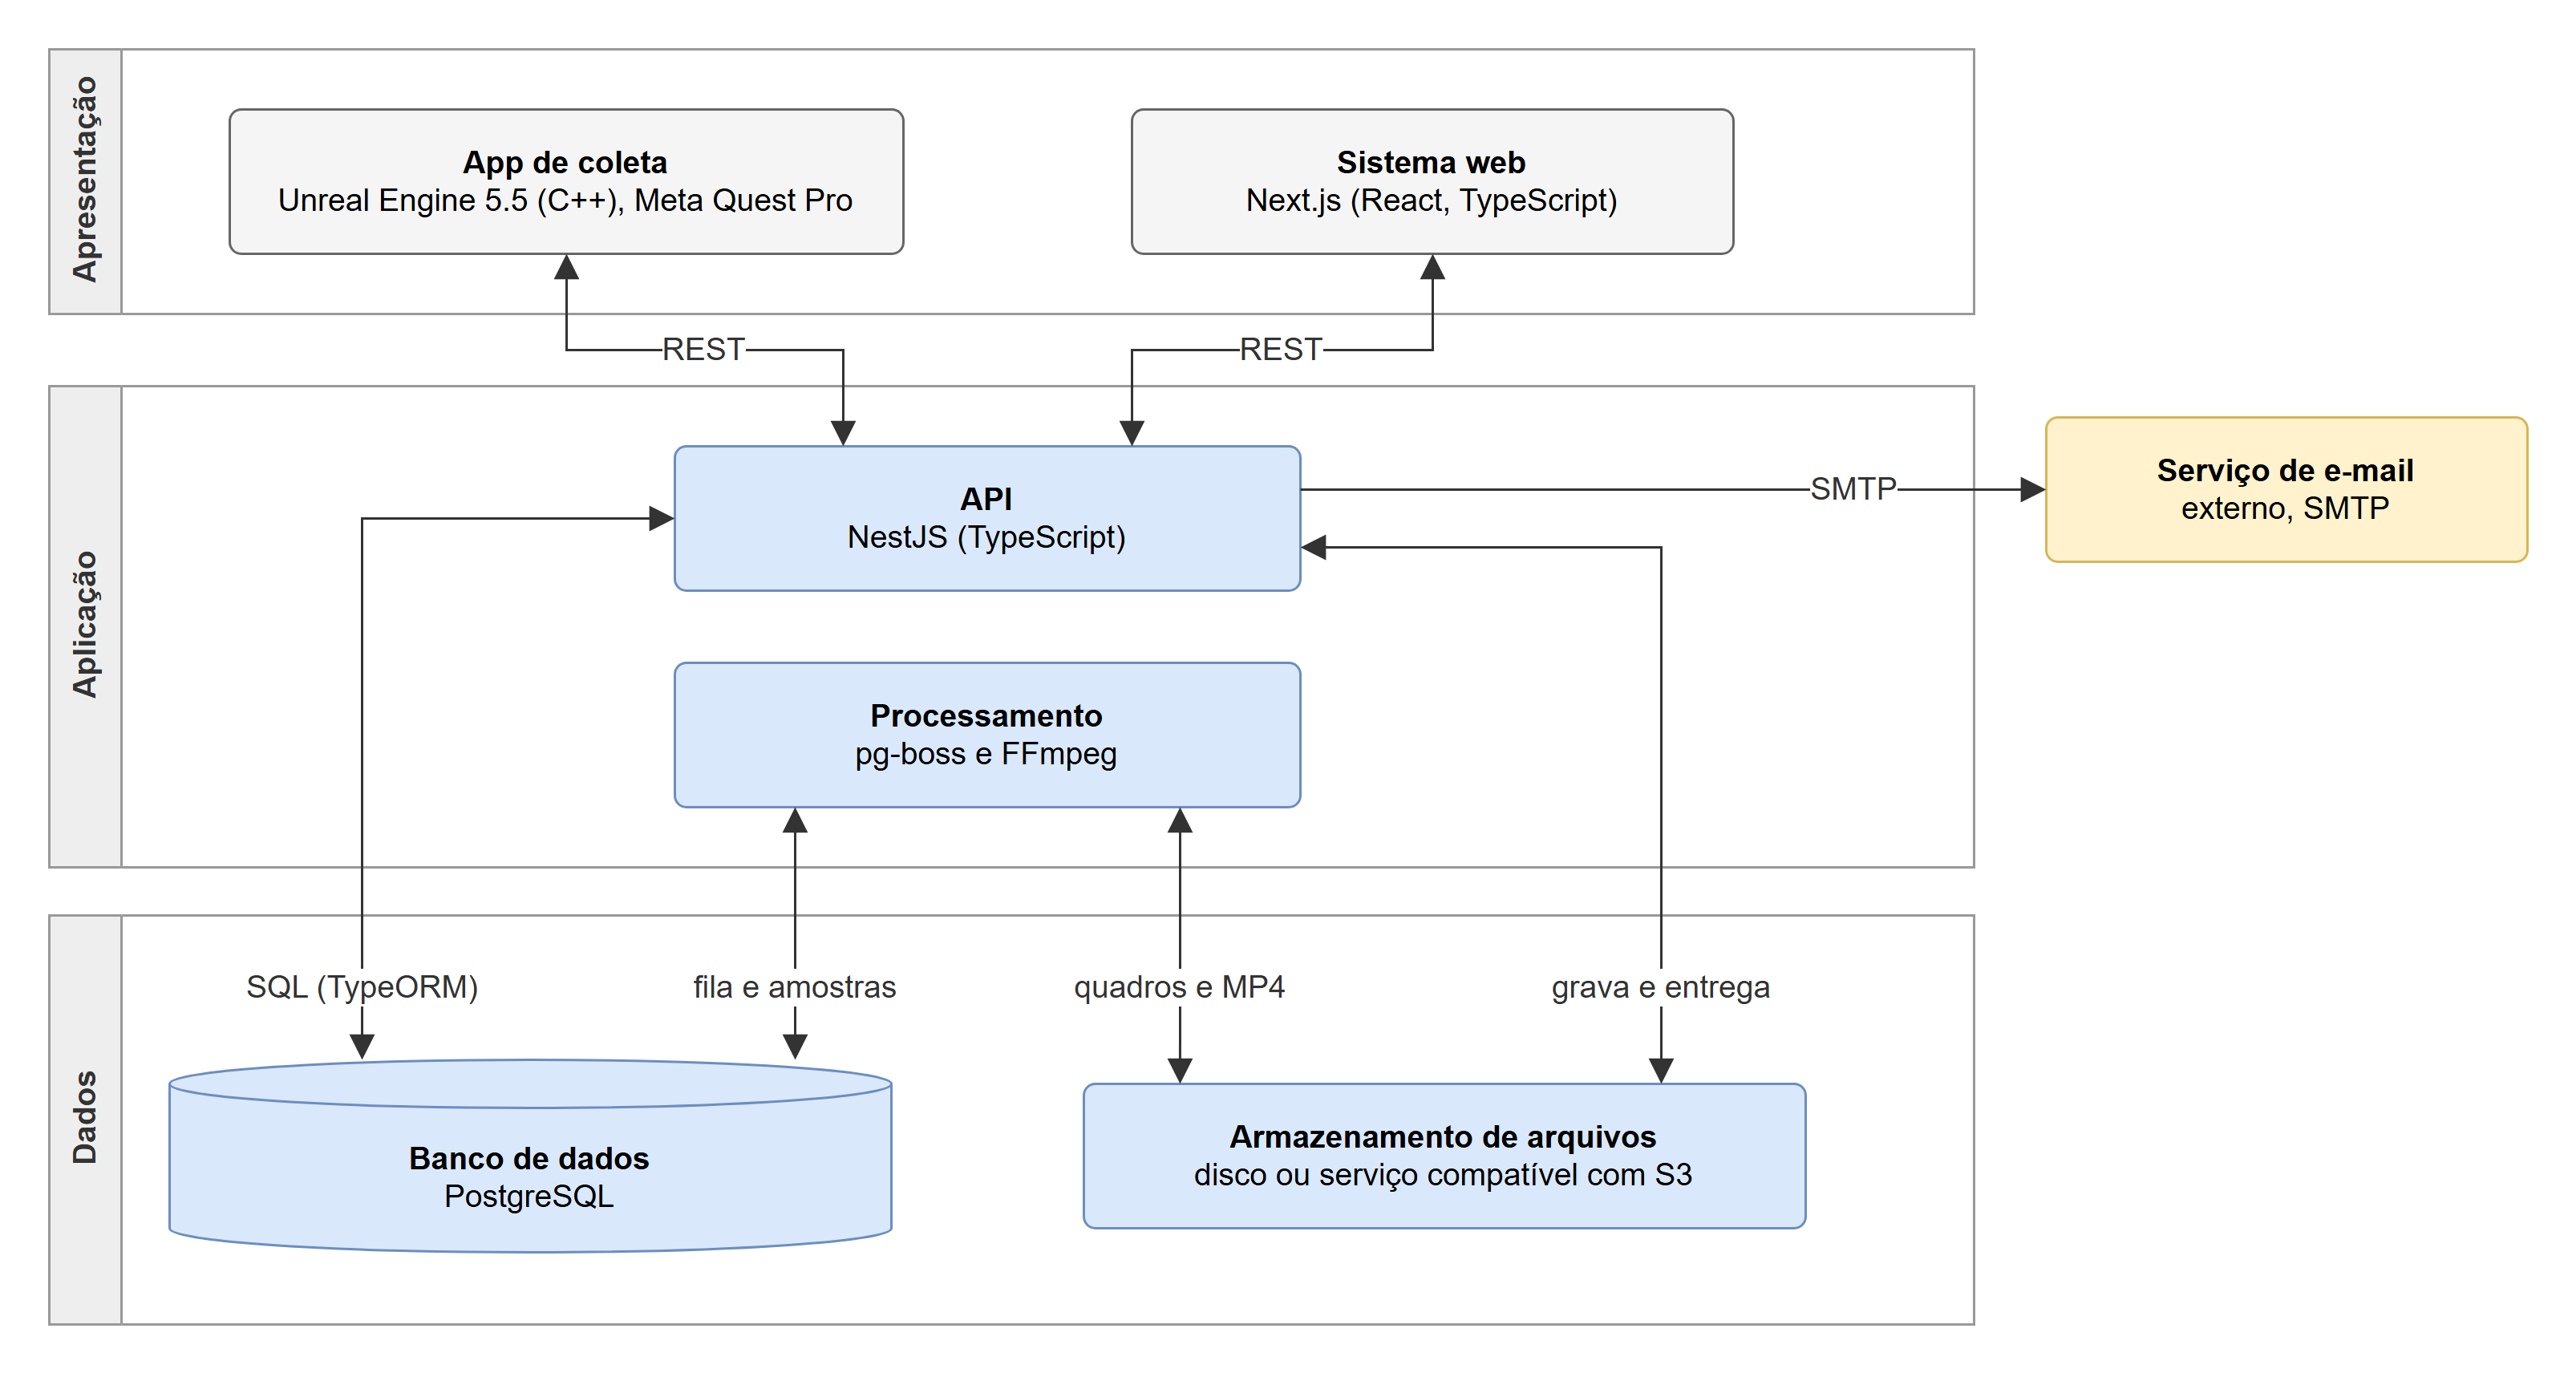
\includegraphics[width=\textwidth]{figuras/Figura-1-arquitetura.png}
\end{figuralarga}

Na Figura 1, observa-se o aplicativo de coleta, desenvolvido a partir do protótipo da IC, que baixa a sessão e os estímulos, apresenta os estímulos ao paciente, coleta o olhar e as expressões faciais, captura os quadros da cena e envia os dados ao servidor. O sistema web é a interface dos pesquisadores e dos administradores e não contém regras de negócio. Essas regras ficam na API, que também é responsável pela autenticação, pelo isolamento entre os grupos de pesquisa, pelo registro de auditoria e pela entrega dos arquivos. A API acessa o banco de dados por meio do TypeORM e guarda os arquivos (estímulos, dados brutos das sessões, quadros e vídeos) no disco do servidor, atrás de uma interface que permite trocar o disco por um serviço de armazenamento compatível com o Amazon S3 sem alterar o restante do sistema. O processamento é executado em segundo plano, a partir de uma fila de tarefas mantida no próprio banco pela biblioteca pg-boss~\cite{PGBOSS}: ele importa as amostras de cada sessão para o banco e monta o vídeo com o FFmpeg. Por fim, um serviço externo de e-mail envia as mensagens de confirmação de cadastro, de convite e de redefinição de senha.

Os componentes do servidor rodam em contêineres, orquestrados pelo Docker Compose, com um \textit{proxy} reverso responsável pela conexão segura (HTTPS, do inglês \textit{Hypertext Transfer Protocol Secure}). Assim, o sistema pode ser instalado em um servidor virtual privado (VPS, do inglês \textit{Virtual Private Server}) contratado, de preferência hospedado no Brasil, ou em um servidor da própria instituição de pesquisa. A escolha cabe ao protocolo de cada pesquisa, aprovado pelo Comitê de Ética em Pesquisa (CEP), já que o art. 13 da LGPD prevê que os dados de estudos em saúde pública sejam tratados dentro do órgão de pesquisa~\cite{LGPD}. O banco de dados e os arquivos terão cópia de segurança diária. Não há comunicação direta entre o sistema web e o óculos: as duas partes falam apenas com a API, como detalhado a seguir.

Cada instituição ou grupo de pesquisa cadastrado no NeuroSight corresponde a um \textit{tenant}, e uma única instalação atende a todos. Os dados ficam em um banco único, em que toda tabela com dados de um \textit{tenant} tem a coluna \texttt{tenant\_id}. O isolamento é feito em duas camadas. Na primeira, a API filtra cada consulta pelo \textit{tenant} do usuário, informado no \textit{token} de acesso. Na segunda, o PostgreSQL aplica em cada tabela uma política de \textit{Row-Level Security} (RLS)~\cite{POSTGRES}, que só devolve as linhas do \textit{tenant} definido para a transação em curso. Assim, um filtro esquecido no código não expõe dados de outro grupo. Como a checagem de chaves estrangeiras não passa pelo RLS, as relações entre as tabelas usam chaves compostas com o \textit{tenant}, o que impede, por exemplo, que uma sessão aponte para o paciente de outro grupo. A API acessa o banco com um papel que não pode ignorar o RLS; um segundo papel, que pode, é usado apenas nas operações feitas antes de existir um \textit{tenant} no contexto, como o autocadastro, o \textit{login} e o pareamento dos óculos. Os arquivos também são separados em pastas por \textit{tenant} e só são entregues pela API, depois da checagem de permissão.

O sistema web e o aplicativo do óculos se comunicam apenas com a API, por HTTPS, no estilo REST (\textit{Representational State Transfer}). A API será documentada em OpenAPI~\cite{OPENAPI}, que serve de contrato entre o servidor e o aplicativo. A Figura 2 resume o fluxo de uma sessão, com os passos numerados na ordem em que ocorrem.

\begin{figuralarga}[!t]{Fluxo de uma sessão no NeuroSight}{Os autores (2026)}{fig:2}
  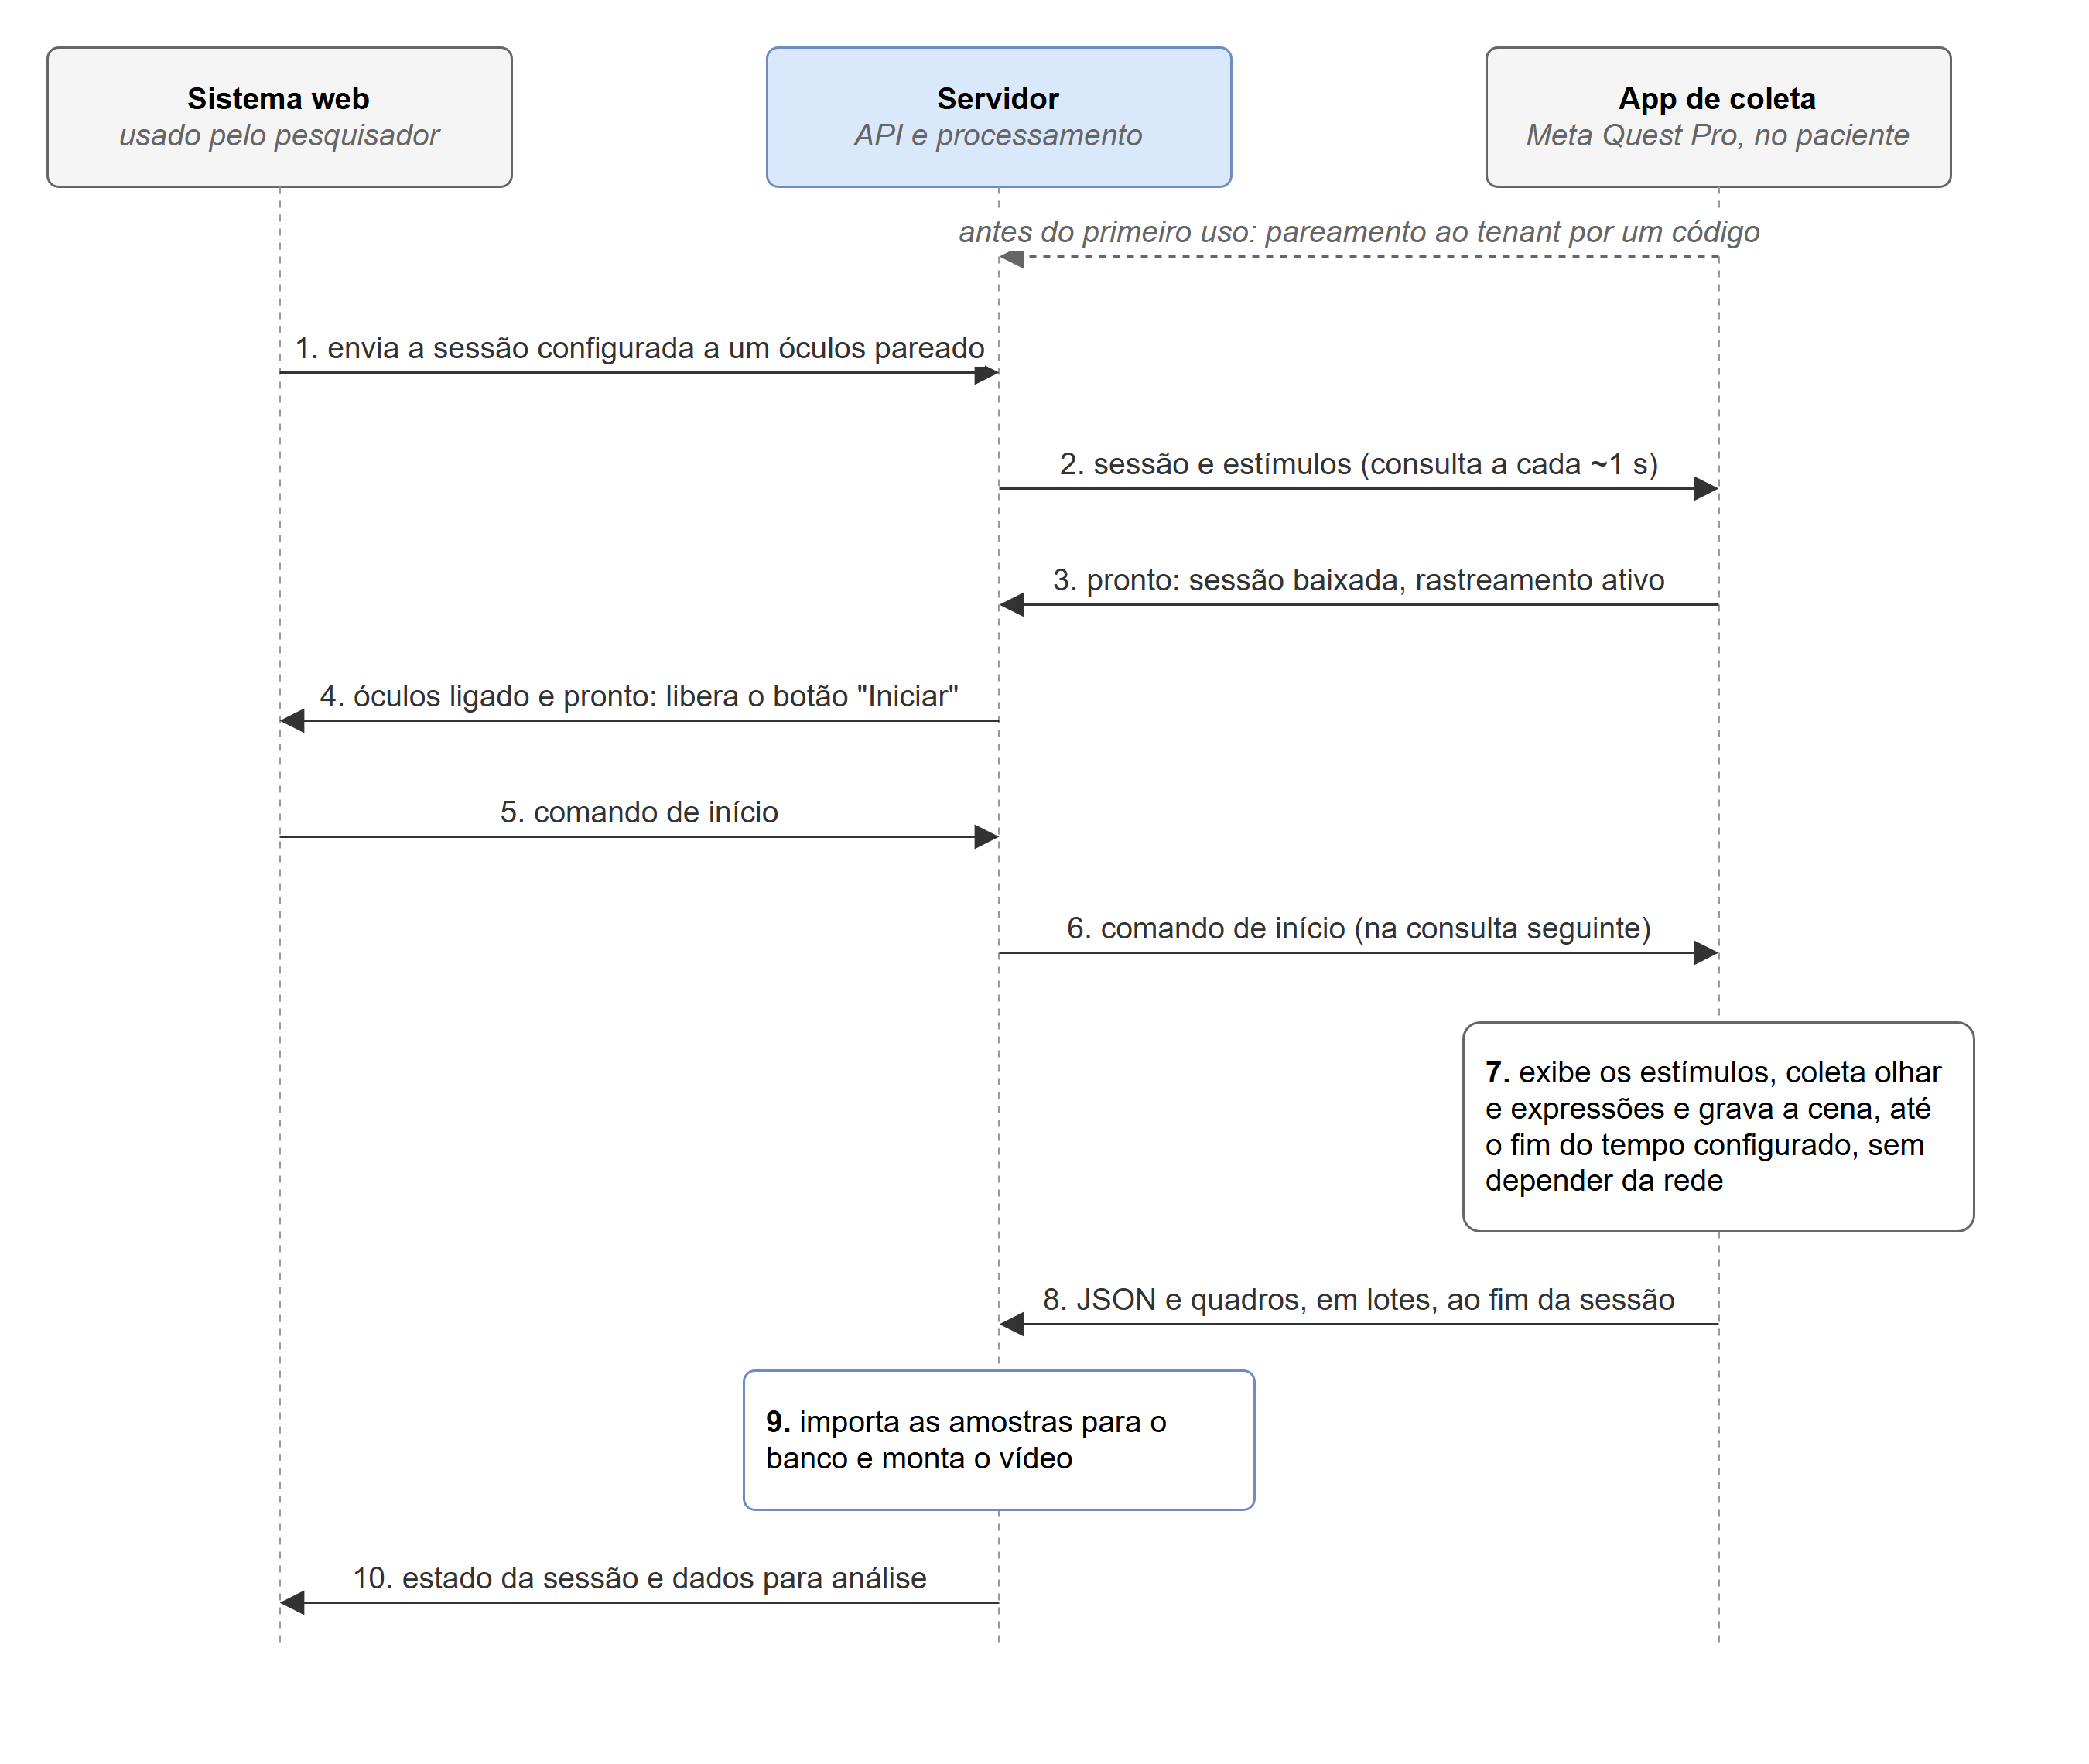
\includegraphics[width=\textwidth]{figuras/Figura-2-fluxo-de-uma-sessao.png}
\end{figuralarga}

Antes do primeiro uso, cada óculos é pareado ao \textit{tenant}. O aplicativo pede ao servidor um código curto, que exibe na tela, e recebe também um segredo. Um administrador digita o código no sistema web e, a partir daí, o segredo passa a valer como \textit{token} de acesso do aparelho, que pode ser revogado a qualquer momento. O mecanismo simplifica o fluxo de autorização de dispositivos do OAuth 2.0~\cite{RFC8628} e dispensa digitar senhas no óculos.

Para executar uma sessão, o pesquisador a configura no sistema web e a envia a um óculos pareado. Enquanto aguarda, o aplicativo consulta o servidor a cada segundo, aproximadamente. Essa mesma consulta indica que o aparelho está ligado, entrega a sessão e transmite o comando de início. Ao receber a sessão, o aplicativo baixa os estímulos que ainda não tem, verifica se o rastreamento ocular e o facial estão ativos e avisa o servidor de que está pronto; só então o sistema web libera o botão ``Iniciar''. Com o óculos já posicionado no paciente, o pesquisador clica em ``Iniciar'', e o aplicativo começa a sessão na consulta seguinte, em até cerca de 2 segundos. Daí em diante, a execução não depende da rede: a sessão segue até o fim do tempo configurado, sem interrupção, e os dados são gravados no próprio óculos.

Optou-se por não espelhar no sistema web a imagem vista pelo paciente: o pesquisador acompanha o estado da sessão e analisa os dados depois que ela termina. Com isso, a comunicação dispensa conexões permanentes, como as de WebSocket, e o óculos e o computador do pesquisador não precisam estar na mesma rede, bastando acesso à internet. Em contrapartida, o óculos precisa estar conectado no momento do início.

Para o controle de acesso, toda comunicação usa HTTPS, e toda chamada à API exige um \textit{token}: um JSON Web Token (JWT)~\cite{JWT}, que identifica o usuário, o \textit{tenant} e o perfil, ou o \textit{token} próprio de cada óculos. As senhas são guardadas apenas na forma de \textit{hash}. A API valida o \textit{token} em cada requisição e usa o perfil nele contido para autorizar ou negar o acesso a cada rota, o que implementa um controle de acesso baseado em papéis. Os perfis são cumulativos: o administrador pode tudo o que o pesquisador pode, e o proprietário, tudo o que o administrador pode.

\subsection{Regras de Negócio e Processamento dos Dados}

Além das funcionalidades de cadastro e de consulta, o sistema implementa um conjunto de regras de negócio que garantem a consistência das sessões e dos dados coletados e automatizam o processamento. As principais são descritas a seguir; a lista completa, com as 20 regras, está na Especificação Técnica.

Toda sessão pertence a exatamente um paciente e é um fluxo de imagens e vídeos exibidos em sequência, cada um pelo tempo definido na configuração; a sessão pode ser criada a partir de um modelo reutilizável ou montada de forma personalizada, e alterar um modelo não altera as sessões já criadas a partir dele. Um estímulo pessoal, como a foto de um familiar, só pode ser usado em sessões do paciente ao qual pertence, e um estímulo já usado em alguma sessão não pode ser excluído, apenas arquivado. Uma sessão só pode ser enviada a um óculos pareado ao mesmo \textit{tenant}, e cada óculos tem no máximo uma sessão pendente por vez. Ao longo do processo, a sessão passa pelos estados rascunho, enviada ao óculos, baixada, início solicitado, em execução, enviando, processando e concluída, ou falha, que o sistema web exibe ao pesquisador. Depois do envio ao óculos, a sessão não pode mais ser editada; para mudá-la, é preciso cancelá-la, o que a devolve a rascunho. O botão ``Iniciar'' só fica liberado quando o óculos de destino está ligado e já baixou a sessão e, depois do início, a sessão sempre vai até o fim do tempo configurado: não há interrupção pelo sistema. Se for preciso retirar o óculos do paciente antes do fim, o pesquisador registra o ocorrido nas anotações da sessão.

Durante a sessão, o aplicativo registra três tipos de dado, todos marcados pelo mesmo relógio do óculos. O primeiro são os eventos de estímulo, com o instante real em que cada estímulo começou e terminou de ser exibido, que pode diferir do tempo configurado, por exemplo, enquanto um vídeo carrega. O segundo é o olhar, amostrado a cada quadro de renderização, com a validade, a confiança, o ponto observado na cena e a sua posição tanto na imagem gravada quanto no próprio estímulo. O terceiro são as expressões faciais: cerca de 70 expressões baseadas no FACS~\cite{EKMAN}, fornecidas pelo kit de desenvolvimento (SDK, do inglês \textit{Software Development Kit}) da Meta~\cite{META-MOVE}, cada uma com intensidade de 0 a 1 e indicação de validade. Esses dados formam um arquivo JSON (\textit{JavaScript Object Notation}), gravado em intervalos curtos para não se perderem caso o aplicativo seja fechado. Como na IC, o aplicativo também captura quadros da cena exibida ao paciente, em JPEG, que servem para montar o vídeo da sessão.

Ao fim da sessão, o aplicativo envia primeiro o JSON e depois os quadros, em lotes. Um lote que falha é reenviado, e um lote repetido não duplica dados. Sem conexão, os dados ficam guardados no óculos, que tenta o envio de novo mais tarde, e só são apagados do aparelho depois que o servidor confirma o recebimento. No servidor, o processamento importa os eventos e as amostras do JSON para tabelas do banco, o que facilita os gráficos e o resumo por estímulo, e monta o vídeo MP4, em H.264, com o FFmpeg. O JSON original é guardado sem alterações, e os dados coletados não podem ser modificados: o pesquisador registra apenas anotações e dados descritivos da sessão. Na IC, cada minuto de gravação, a cerca de 22 quadros por segundo, gerou aproximadamente 88 MB~\cite{IC}. Com base nessa medição, estima-se que uma sessão de 5 minutos, com quadros de 1024 $\times$ 1024 pixels capturados a 15 quadros por segundo, gere cerca de 300 MB, valor que será medido no NeuroSight.

Com a sessão concluída, o sistema web reproduz o vídeo com o mapa de calor do olhar, cuja janela temporal, raio e opacidade o pesquisador ajusta durante a reprodução; oferece um modo de validação, com o ponto do olhar desenhado sobre o vídeo; exibe os gráficos das expressões faciais ao longo do tempo, com a marcação de cada estímulo; e calcula um resumo por estímulo, com o tempo de olhar dentro do estímulo, a porcentagem de amostras válidas e a intensidade média das expressões, a partir dos instantes reais registrados no óculos. Os dados de uma sessão só ficam visíveis para quem a criou, para o proprietário, para os administradores e para os usuários que um administrador autorizar. O sistema registra automaticamente quem fez cada ação, quando e em qual registro, abrangendo \textit{login}, criação, edição e exclusão de dados, envio e início de sessões, visualização e exportação dos dados de uma sessão e mudanças de permissão. Os registros de auditoria não podem ser alterados nem excluídos, restrição garantida no próprio banco, pois o papel usado pela API não tem permissão para isso.

Os dados de saúde são dados pessoais sensíveis segundo a LGPD~\cite{LGPD}, e o sistema foi modelado para guardar apenas o necessário à pesquisa. O paciente é identificado por um código; o nome é opcional e nunca chega ao óculos, que exibe só o código. O aplicativo não captura imagens do rosto do paciente, apenas os valores das expressões, e a gravação mostra somente o que o paciente viu. O consentimento para a participação, dado pelo representante legal do paciente, fica a cargo do protocolo de cada pesquisa, aprovado pelo CEP, e não é tratado pelo sistema.

\section{CONSIDERAÇÕES FINAIS}

Este trabalho apresentou a modelagem do NeuroSight, um sistema de apoio à pesquisa com pessoas com distúrbios da consciência que reúne, em uma única ferramenta, as etapas dos experimentos com rastreamento ocular e expressões faciais em realidade virtual: o cadastro de pacientes e de estímulos, a configuração e o início das sessões pelo sistema web, a coleta no Meta Quest Pro, o envio e o processamento dos dados e a sua análise. A revisão de literatura confirmou que o rastreamento ocular detecta mais respostas do que a observação clínica nesses pacientes, que estímulos com significado pessoal tendem a provocar mais respostas do que estímulos neutros e que as ferramentas disponíveis não reúnem a coleta do olhar e das expressões faciais no Meta Quest Pro, a apresentação de uma sequência de estímulos com tempo definido e o armazenamento centralizado dos dados de vários grupos de pesquisa, com controle de acesso e auditoria. A proposta parte do protótipo desenvolvido na Iniciação Científica, cujo aplicativo e cuja forma de gravação das sessões são reaproveitados.

A etapa de modelagem produziu 60 requisitos funcionais, 20 regras de negócio e 26 requisitos não funcionais; doze diagramas de casos de uso, com 60 casos de uso, e as 60 histórias de usuário correspondentes; o diagrama de classes; o diagrama de estados da sessão; seis diagramas de sequência; o modelo lógico do banco de dados, com 20 tabelas; dois diagramas de processo de negócio; e 19 protótipos de tela, todos reunidos na Especificação Técnica que acompanha este artigo. A arquitetura definida, com um aplicativo em Unreal Engine, uma API em NestJS, um sistema web em Next.js e um banco de dados PostgreSQL compartilhado por vários grupos de pesquisa, com isolamento por \textit{Row-Level Security}, controle de acesso e auditoria, atende aos requisitos de proteção dos dados de saúde e serve de base para o desenvolvimento. Do ponto de vista metodológico, o Scrum adaptado a uma equipe de dois integrantes, com o quadro Kanban no GitHub Projects e as reuniões de orientação, organizou o trabalho e permitiu validar as decisões ao longo da modelagem.

Cabe ressaltar que este trabalho concentrou-se no levantamento de requisitos, na modelagem e no projeto da arquitetura, não incluindo ainda a implementação. Três pontos da arquitetura dependem de verificação na etapa seguinte. O primeiro é a leitura das expressões faciais no Unreal Engine: o protótipo da IC lê apenas o olhar, pelo padrão OpenXR, e as opções de rastreamento da Meta, que fornecem as expressões, exigem outra integração do motor, incompatível com a usada no protótipo~\cite{IC}. Por isso, a primeira tarefa do desenvolvimento será uma prova de conceito que leia o olhar e as expressões ao mesmo tempo e meça a taxa de amostragem obtida com a captura de quadros ativa, que na IC ficou em 22 Hz~\cite{IC}; se a prova de conceito falhar, a alternativa é desenvolver o aplicativo em Unity, em que o olhar e as expressões vêm do mesmo SDK. O segundo ponto é o equipamento: o Meta Quest Pro saiu de linha em janeiro de 2025~\cite{HAYDEN} e, embora o grupo de pesquisa disponha do aparelho usado na IC, a reposição, em caso de defeito, seria difícil. O terceiro é a dependência de internet no momento do início da sessão, já que o comando sai do sistema web e chega ao óculos pelo servidor; por isso, a rede do local da coleta precisa ser testada antes dos experimentos.

As etapas seguintes envolvem a prova de conceito, o desenvolvimento do aplicativo, da API e do sistema web em \textit{sprints}, a partir do \textit{backlog} formado pelas histórias de usuário, a medição do volume de dados de uma sessão real, estimado em cerca de 300 MB para 5 minutos, e os testes do sistema com o óculos. O uso com pacientes depende da aprovação de um protocolo de pesquisa pelo Comitê de Ética em Pesquisa, com o consentimento dos representantes legais, e da escolha da hospedagem conforme esse protocolo. O NeuroSight não faz diagnóstico nem substitui a avaliação clínica: a expectativa é que, ao organizar os experimentos e o registro dos dados, ele facilite a pesquisa sobre as respostas visuais e emocionais dessas pessoas e contribua, no futuro, para o apoio ao diagnóstico.


%%%%%%%%%%%%%%%%%%%%%%%%%%%%%%%%%%%%%%%%%%%%%%%%%%%%%%%%%%%%
% REFERÊNCIAS (já na ordem da primeira citação, como no artigo montado)

\def\refname{Referências}

\begin{thebibliography}{99}

\bibitem{LAUREYS} LAUREYS, S. \textit{et al}. Unresponsive wakefulness syndrome: a new name for the vegetative state or apallic syndrome. \textit{BMC Medicine}, v. 8, art. 68, 2010. DOI: 10.1186/1741-7015-8-68.

\bibitem{GIACINO2002} GIACINO, J. T. \textit{et al}. The minimally conscious state: definition and diagnostic criteria. \textit{Neurology}, v. 58, n. 3, p. 349-353, 2002. DOI: 10.1212/WNL.58.3.349.

\bibitem{GIACINO2004} GIACINO, J. T.; KALMAR, K.; WHYTE, J. The JFK Coma Recovery Scale-Revised: measurement characteristics and diagnostic utility. \textit{Archives of Physical Medicine and Rehabilitation}, v. 85, n. 12, p. 2020-2029, 2004. DOI: 10.1016/j.apmr.2004.02.033.

\bibitem{SCHNAKERS} SCHNAKERS, C. \textit{et al}. Diagnostic accuracy of the vegetative and minimally conscious state: clinical consensus versus standardized neurobehavioral assessment. \textit{BMC Neurology}, v. 9, art. 35, 2009. DOI: 10.1186/1471-2377-9-35.

\bibitem{BODIEN} BODIEN, Y. G. \textit{et al}. Cognitive motor dissociation in disorders of consciousness. \textit{New England Journal of Medicine}, v. 391, n. 7, p. 598-608, 2024. DOI: 10.1056/NEJMoa2400645.

\bibitem{TROJANO} TROJANO, L. \textit{et al}. Quantitative assessment of visual behavior in disorders of consciousness. \textit{Journal of Neurology}, v. 259, n. 9, p. 1888-1895, 2012. DOI: 10.1007/s00415-012-6435-4.

\bibitem{EKMAN} EKMAN, P.; FRIESEN, W. V. \textit{Facial Action Coding System: a technique for the measurement of facial movement}. Palo Alto: Consulting Psychologists Press, 1978.

\bibitem{MAGLIACANO} MAGLIACANO, A. \textit{et al}. Can salient stimuli enhance responses in disorders of consciousness? A systematic review. \textit{Current Neurology and Neuroscience Reports}, v. 19, n. 12, art. 98, 2019. DOI: 10.1007/s11910-019-1018-8.

\bibitem{CLAY} CLAY, V.; KÖNIG, P.; KÖNIG, S. U. Eye tracking in virtual reality. \textit{Journal of Eye Movement Research}, v. 12, n. 1, 2019. DOI: 10.16910/jemr.12.1.3.

\bibitem{META-MOVE} META PLATFORMS. \textit{Movement SDK for Unreal}. Meta Horizon OS Developers, 2026. Disponível em: \url{https://developers.meta.com/vr/documentation/unreal/unreal-movement-overview/}. Acesso em: 26 out. 2026.

\bibitem{JOHANSSON} JOHANSSON, J. \textit{et al}. Eye tracking to support assessment of patients with prolonged disorder of consciousness: a case series. \textit{Journal of Rehabilitation Medicine}, v. 57, art. jrm41324, 2025. DOI: 10.2340/jrm.v57.41324.

\bibitem{HYUN} HYUN, C. \textit{et al}. Quantitative evaluation of the consciousness level of patients in a vegetative state using virtual reality and an eye-tracking system: a single-case experimental design study. \textit{Neuropsychological Rehabilitation}, v. 32, n. 10, p. 2628-2645, 2022. DOI: 10.1080/09602011.2021.1974496.

\bibitem{IC} PEDRO, J. V. Z. \textit{Desenvolvimento de um sistema de rastreamento ocular em realidade virtual para análise de atenção visual aplicada ao estudo da recepção comunicacional}. Relatório final de Iniciação Científica (Edital 2025) -- Universidade Federal do Paraná, Curitiba, 2026. Orientador: Alessandro Brawerman. Disponível em: \url{https://github.com/joaozanini/QuestPro-EyeTracking}. Acesso em: 26 out. 2026.

\bibitem{LGPD} BRASIL. \textit{Lei nº 13.709, de 14 de agosto de 2018}. Lei Geral de Proteção de Dados Pessoais (LGPD). Brasília, DF: Presidência da República, [2018]. Disponível em: \url{https://www.planalto.gov.br/ccivil_03/_ato2015-2018/2018/lei/l13709compilado.htm}. Acesso em: 26 out. 2026.

\bibitem{ESTRANEO} ESTRANEO, A. \textit{et al}. Eye-tracking assessment in patients with disorders of consciousness: a systematic review. \textit{Brain Sciences}, v. 16, n. 6, art. 590, 2026. DOI: 10.3390/brainsci16060590.

\bibitem{BAGNATO} BAGNATO, S.; BOCCAGNI, C.; BONAVITA, J. Eye movements as indicators of awareness in prolonged disorders of consciousness: a scoping review of behavioral and neural evidence. \textit{Neurological Sciences}, v. 47, n. 3, art. 317, 2026. DOI: 10.1007/s10072-026-08932-6.

\bibitem{PICARD} PICARD, R. W. \textit{Affective computing}. Cambridge: MIT Press, 1997. DOI: 10.7551/mitpress/1140.001.0001.

\bibitem{META-FACE-PRIV} META PLATFORMS. \textit{Natural Facial Expressions Privacy Notice}. 5 set. 2025. Disponível em: \url{https://www.meta.com/legal/quest/natural-facial-expressions-privacy-notice/}. Acesso em: 26 out. 2026.

\bibitem{IMOTIONS-PRICE} IMOTIONS. \textit{iMotions Lab Pricing}. Disponível em: \url{https://imotions.com/products/pricing/}. Acesso em: 26 out. 2026.

\bibitem{IMOTIONS-FEA} IMOTIONS. \textit{Facial Expression Analysis}: emotion detection software. Disponível em: \url{https://imotions.com/products/imotions-lab/modules/fea-facial-expression-analysis/}. Acesso em: 26 out. 2026.

\bibitem{IMOTIONS-SB} IMOTIONS. \textit{Study Builder}. Disponível em: \url{https://imotions.com/products/imotions-lab/features/study-builder/}. Acesso em: 26 out. 2026.

\bibitem{IMOTIONS-NEWS} IMOTIONS. \textit{iMotions Product \& Feature News}: February 2026. 2026. Disponível em: \url{https://imotions.com/about-us/news/imotions-product-feature-news-february-2026/}. Acesso em: 26 out. 2026.

\bibitem{IMOTIONS-TOS} IMOTIONS. \textit{Terms of Service}. Disponível em: \url{https://imotions.com/terms-of-service/}. Acesso em: 26 out. 2026.

\bibitem{SIGHTLAB} WORLDVIZ. \textit{What is SightLab VR Pro and how does it work?} 2025. Disponível em: \url{https://www.worldviz.com/post/what-is-sightlab-vr-pro-and-how-does-it-work}. Acesso em: 26 out. 2026.

\bibitem{WORLDVIZ-PRICE} WORLDVIZ. \textit{2026 WorldViz VR budgeting guidelines for scientific VR labs}. 2026. Disponível em: \url{https://www.worldviz.com/post/worldviz-vr-budgeting-guidelines-for-scientific-vr-labs}. Acesso em: 26 out. 2026.

\bibitem{SIGHTLAB-FACE} WORLDVIZ. \textit{Face Tracking}: SightLab documentation. Disponível em: \url{https://help.worldviz.com/sightlab/face-tracking}. Acesso em: 26 out. 2026.

\bibitem{SIGHTLAB-MEDIA} WORLDVIZ. \textit{Media Viewer}: SightLab documentation. Disponível em: \url{https://help.worldviz.com/sightlab/media-viewer/}. Acesso em: 26 out. 2026.

\bibitem{COG3D-PRICING} COGNITIVE3D. \textit{XR Analytics Platform Pricing}. Disponível em: \url{https://cognitive3d.com/pricing/}. Acesso em: 26 out. 2026.

\bibitem{COG3D-CONCEPTS} COGNITIVE3D. \textit{Concepts}: Cognitive3D documentation. Disponível em: \url{https://docs.cognitive3d.com/dashboard/concepts/}. Acesso em: 26 out. 2026.

\bibitem{COG3D-HARDWARE} COGNITIVE3D. \textit{Supported Hardware}: Cognitive3D documentation. Disponível em: \url{https://docs.cognitive3d.com/hardware/}. Acesso em: 2 nov. 2026.

\bibitem{COG3D-DPA} COGNITIVE3D. \textit{Data Processing Addendum}. Disponível em: \url{https://cognitive3d.com/dpa/}. Acesso em: 26 out. 2026.

\bibitem{SCRUM} SCHWABER, K.; SUTHERLAND, J. \textit{The Scrum Guide}. [S.l.]: Scrum.org, 2020. E-book. Disponível em: \url{https://scrumguides.org/docs/scrumguide/v2020/2020-Scrum-Guide-US.pdf}. Acesso em: 26 out. 2026.

\bibitem{KANBAN} ANDERSON, D. J. \textit{Kanban: successful evolutionary change for your technology business}. Sequim: Blue Hole Press, 2010.

\bibitem{GITHUB} GITHUB. \textit{Planning and tracking with Projects}. 2026. Disponível em: \url{https://docs.github.com/en/issues/planning-and-tracking-with-projects}. Acesso em: 26 out. 2026.

\bibitem{UML} OBJECT MANAGEMENT GROUP. \textit{OMG Unified Modeling Language (OMG UML)}: version 2.5.1. Needham: OMG, 2017. Disponível em: \url{https://www.omg.org/spec/UML/2.5.1/}. Acesso em: 26 out. 2026.

\bibitem{BPMN} OBJECT MANAGEMENT GROUP. \textit{Business Process Model and Notation (BPMN)}: version 2.0.2. Needham: OMG, 2013. Disponível em: \url{https://www.omg.org/spec/BPMN/2.0.2/}. Acesso em: 26 out. 2026.

\bibitem{DRAWIO} JGRAPH. \textit{draw.io}. 2026. Disponível em: \url{https://www.drawio.com/}. Acesso em: 26 out. 2026.

\bibitem{COHN} COHN, M. \textit{User stories applied: for agile software development}. Boston: Addison-Wesley, 2004.

\bibitem{UNREAL} EPIC GAMES. \textit{Unreal Engine 5.5 documentation}. 2025. Disponível em: \url{https://dev.epicgames.com/documentation/en-us/unreal-engine/unreal-engine-5-5-documentation}. Acesso em: 26 out. 2026.

\bibitem{OPENXR} KHRONOS GROUP. \textit{OpenXR registry}. 2026. Disponível em: \url{https://registry.khronos.org/OpenXR/}. Acesso em: 26 out. 2026.

\bibitem{META-UNREAL} META PLATFORMS. \textit{Unreal integration: settings and tools}. Meta Horizon OS Developers, 2026. Disponível em: \url{https://developers.meta.com/vr/documentation/unreal/}. Acesso em: 26 out. 2026.

\bibitem{TYPESCRIPT} MICROSOFT. \textit{TypeScript documentation}. 2026. Disponível em: \url{https://www.typescriptlang.org/docs/}. Acesso em: 26 out. 2026.

\bibitem{NESTJS} NESTJS. \textit{NestJS documentation}. 2026. Disponível em: \url{https://docs.nestjs.com/}. Acesso em: 26 out. 2026.

\bibitem{TYPEORM} TYPEORM. \textit{TypeORM documentation}. 2026. Disponível em: \url{https://typeorm.io/docs/getting-started}. Acesso em: 26 out. 2026.

\bibitem{POSTGRES} POSTGRESQL GLOBAL DEVELOPMENT GROUP. \textit{PostgreSQL documentation: row security policies}. 2026. Disponível em: \url{https://www.postgresql.org/docs/current/ddl-rowsecurity.html}. Acesso em: 26 out. 2026.

\bibitem{NEXTJS} VERCEL. \textit{Next.js documentation}. 2026. Disponível em: \url{https://nextjs.org/docs}. Acesso em: 26 out. 2026.

\bibitem{FFMPEG} FFMPEG. \textit{FFmpeg documentation}. 2026. Disponível em: \url{https://ffmpeg.org/documentation.html}. Acesso em: 26 out. 2026.

\bibitem{DOCKER} DOCKER. \textit{Docker Compose documentation}. 2026. Disponível em: \url{https://docs.docker.com/compose/}. Acesso em: 26 out. 2026.

\bibitem{GIT} GIT. \textit{Git SCM}. 2026. Disponível em: \url{https://git-scm.com/}. Acesso em: 26 out. 2026.

\bibitem{PGBOSS} PG-BOSS. \textit{pg-boss: queueing jobs in Postgres from Node.js}. GitHub, 2026. Disponível em: \url{https://github.com/timgit/pg-boss}. Acesso em: 26 out. 2026.

\bibitem{OPENAPI} OPENAPI INITIATIVE. \textit{OpenAPI Specification}: version 3.2.1. 2026. Disponível em: \url{https://spec.openapis.org/oas/v3.2.1.html}. Acesso em: 26 out. 2026.

\bibitem{RFC8628} DENNISS, W. \textit{et al}. \textit{OAuth 2.0 Device Authorization Grant}. RFC 8628. [S.l.]: IETF, 2019. Disponível em: \url{https://www.rfc-editor.org/rfc/rfc8628}. Acesso em: 26 out. 2026.

\bibitem{JWT} JONES, M.; BRADLEY, J.; SAKIMURA, N. \textit{JSON Web Token (JWT)}. RFC 7519. [S.l.]: IETF, 2015. Disponível em: \url{https://www.rfc-editor.org/rfc/rfc7519}. Acesso em: 26 out. 2026.

\bibitem{HAYDEN} HAYDEN, S. Meta officially discontinues Quest Pro, its first (and most expensive) mixed reality headset. \textit{Road to VR}, 6 jan. 2025. Disponível em: \url{https://roadtovr.com/meta-discontinues-quest-pro/}. Acesso em: 26 out. 2026.

\end{thebibliography}

\end{document}
